\documentclass[conference]{IEEEtran}
\IEEEoverridecommandlockouts
\usepackage{cite}
\usepackage{amsmath,amssymb,amsfonts}
\usepackage{algorithmic}
\usepackage{graphicx}
\usepackage{textcomp}
\usepackage{xcolor}
\usepackage{url}
\usepackage{hyperref}
\def\BibTeX{{\rm B\kern-.05em{\sc i\kern-.025em b}\kern-.08em
    T\kern-.1667em\lower.7ex\hbox{E}\kern-.125emX}}
\begin{document}

\title{Regresión Lineal Manual: Predicción del Desempeño de Estudiantes}

\author{\IEEEauthorblockN{Fabricio Mena Mejia y Anthony Fuentes Calvo}
\IEEEauthorblockA{
Instituto Tecnológico de Costa Rica\\
Email: fabriciomena11@estudiantec.cr, 2021045930@gmail.com}}

\maketitle

\begin{abstract}
El propósito de esta tarea es implementar y analizar un
modelo de regresión logística para resolver un problema de
clasificación binario para determinar si la calidad de un
vino es ”BUENA” o ”MALA”, utilizando como entorno de
desarrollo PyTorch para la optimización y creación de modelos
personalizados.
Se espera que el estudiante realice un análisis exploratorio
detallado de las características del conjunto de datos y la
variable a predecir, que implemente stratified sampling, ajuste
un modelo de regresión logística y evalúe aplicando métricas.
\end{abstract}

\section{Desarrollo de Regresión Logística con PyTorch}

Para este trabajo se utiliza el conjunto de datos \textit{winequality-red}, que
contiene 1~599 observaciones de vinos tintos descritos por 11 características
fisicoquímicas numéricas y una variable de calidad sensorial
\texttt{quality}, con valores enteros entre 3 y 8. El objetivo es construir un
modelo de regresión logística binaria que clasifique cada vino como
\textbf{BUENO} o \textbf{MALO}.

Se define una variable objetivo binaria $y_{\text{bin}}$ a partir de la
calidad original,
\begin{equation}
    y_{\text{bin}} =
    \begin{cases}
        1, & \text{si } \texttt{quality} \geq 7 \\[2pt]
        0, & \text{en otro caso},
    \end{cases}
\end{equation}
de modo que la clase positiva representa vinos de buena calidad (puntuación 7 u
8). La distribución resultante es desbalanceada, con aproximadamente un
13.6\,\% de vinos de buena calidad y 86.4\,\% de vinos catalogados como
``normales''. Esta proporción se mantiene en todas las particiones mediante
muestreo estratificado.

Antes de ajustar el modelo se realiza un tratamiento de outliers sobre las
seis características seleccionadas ya que algunos boxplots como el de sulfatos y el de la densidad (ver Fig.~\ref{fig:boxplot_sulfate} y Fig.~\ref{fig:boxplot_density} ). En el cuaderno se aplica el criterio del
\textit{rango intercuartílico} (IQR): para cada variable se calculan el primer
cuartil $Q_1$ y el tercer cuartil $Q_3$, y se eliminan las observaciones con
valores fuera del intervalo $[Q_1 - 1.5\,IQR,\, Q_3 + 1.5\,IQR]$, donde
$IQR = Q_3 - Q_1$. Esto reduce ligeramente el número de filas pero mejora la
robustez del ajuste frente a valores extremos detectados en los boxplots.

\begin{figure}[ht]
    \centering
    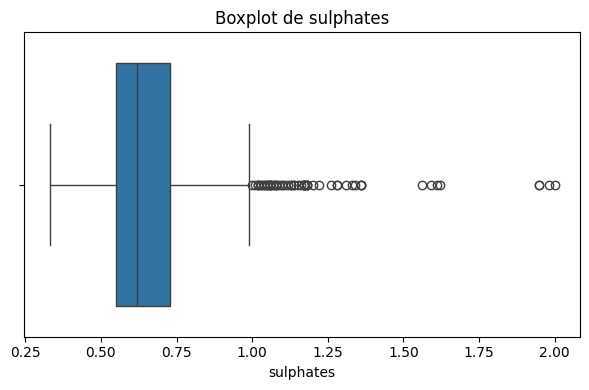
\includegraphics[width=0.9\linewidth]{images/boxplot_sulfate.png}
    \caption{Boxplot de Sulfatos mostrando outliers.}
    \label{fig:boxplot_sulfate}
\end{figure}

\begin{figure}[ht]
    \centering
    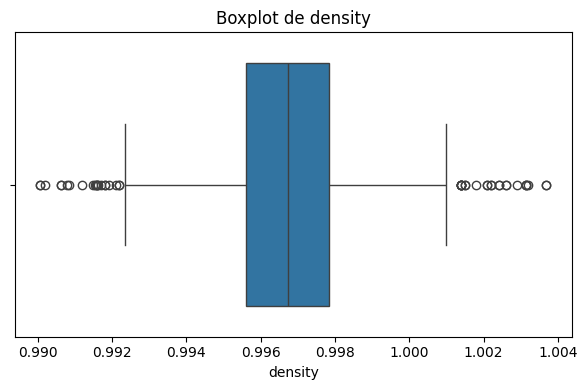
\includegraphics[width=0.9\linewidth]{images/boxplot_density.png}
    \caption{Boxplot de Densidad mostrando outliers.}
    \label{fig:boxplot_density}
\end{figure}

Posteriormente, en el cuaderno \texttt{Tarea2.ipynb} se divide el conjunto de
datos limpio en tres subconjuntos mutuamente excluyentes: 70~\% para
entrenamiento, 15~\% para validación y 15~\% para prueba, utilizando
\texttt{train\_test\_split} con la opción \texttt{stratify} para mantener la
proporción de la clase positiva en cada partición. A continuación se escalan
las seis características seleccionadas mediante \textit{StandardScaler}
(ajustado con los datos de entrenamiento) y se construyen tensores de PyTorch
para alimentar el modelo.

Para garantizar la reproducibilidad de los resultados, en el cuaderno se fijan
las semillas de los generadores pseudoaleatorios de Python, NumPy y PyTorch
(por ejemplo, con una semilla global igual a 42). De este modo, cada vez que
se ejecuta el cuaderno completo se obtienen las mismas particiones y el mismo
comportamiento de entrenamiento para las 10 configuraciones de
hiperparámetros, haciendo que las métricas reportadas sean deterministas.

El clasificador se implementa como una regresión logística clásica en PyTorch
(celda 9). El modelo consta de una única capa lineal con dimensión de entrada
igual al número de características seleccionadas,
\begin{equation}
    z = w^\top x + b, \qquad \hat y = \sigma(z),
\end{equation}
donde $\sigma(\cdot)$ es la función sigmoide. Para el entrenamiento se utiliza
la función de pérdida \textit{Binary Cross-Entropy} con logits
\texttt{BCEWithLogitsLoss} y el optimizador Adam. En cada época se calcula la
pérdida tanto en el conjunto de entrenamiento como en el de validación, lo que
permite analizar gráficamente el comportamiento de \textit{underfitting} u
\textit{overfitting} del modelo.

\section{Justificación de selección de features}

El conjunto original de 11 características se reduce a un máximo de seis para
evitar modelos innecesariamente complejos y cumplir con la consigna. La
selección se basa en dos criterios matemáticos: (i) la correlación lineal con
la variable de calidad y (ii) la multicolinealidad entre predictores.

En primer lugar, se calcula la matriz de correlación de Pearson entre todas las
variables numéricas (celda 2 del notebook). La Fig.~\ref{fig:corr_heatmap}
muestra el mapa de calor de dichas correlaciones, donde puede observarse que el
grado alcohólico, la acidez volátil, los sulfatos, el ácido cítrico, el dióxido
de azufre total y la densidad son las variables con mayor correlación (en
módulo) con la calidad.

\begin{figure}[ht]
    \centering
    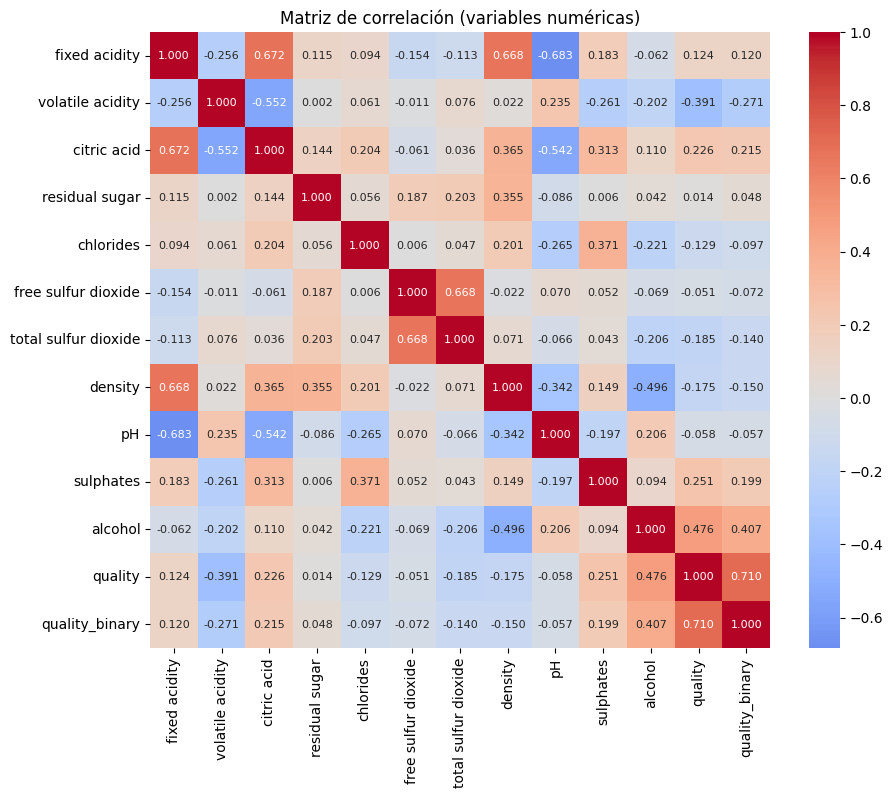
\includegraphics[width=0.9\linewidth]{images/fig_corr_heatmap.png}
    \caption{Matriz de correlación de las variables numéricas del conjunto de
    vinos tintos.}
    \label{fig:corr_heatmap}
\end{figure}

Sea $x_j$ cada característica numérica y $y$ la calidad original. La
correlación de Pearson se define como
\begin{equation}
    r(x_j, y) = \frac{\operatorname{cov}(x_j, y)}{\sigma_{x_j} \, \sigma_y},
\end{equation}
por lo que $|r(x_j, y)|$ mide la fuerza de la relación lineal entre $x_j$ y la
calidad. En la celda 2 se ordenan las características según el valor absoluto
de esta correlación. A continuación, en la celda 3 se recorre esa lista
ordenada y se construye un conjunto de características $S$ de tamaño máximo 6,
aplicando el siguiente procedimiento:

\begin{enumerate}
    \item Inicialmente $S = \varnothing$.
    \item Para cada nueva característica $x_j$ en el orden dado, se calcula su
                correlación con las ya incluidas en $S$.
    \item Si para alguna $s \in S$ se cumple $|r(x_j, s)| > 0.8$, se considera
                que hay multicolinealidad severa y se descarta $x_j$.
    \item En caso contrario, se añade $x_j$ a $S$.
\end{enumerate}

Este algoritmo garantiza que todas las variables de $S$ estén fuertemente
relacionadas con la calidad pero no excesivamente correlacionadas entre sí. El
conjunto final seleccionado es
\begin{equation}
\begin{aligned}
S = \{&\texttt{alcohol},\ \texttt{volatile acidity},\\
     &\texttt{sulphates},\ \texttt{citric acid},\\
     &\texttt{total sulfur dioxide},\ \texttt{density}\}
\end{aligned}
\end{equation}

Para estas seis características se generan histogramas, boxplots y diagramas de
dispersión frente a la calidad original. En los histogramas de alcohol(Fig.~\ref{fig:hist_alcohol}) y acidez volátil(Fig.~\ref{fig:hist_volatile}) podemos ver que la mayor frecuencia de su aparición es en el lado izquierdo, indicando que sus concentraciones suelen ser menores para la mayoría de vinos.

\begin{figure}[ht]
    \centering
    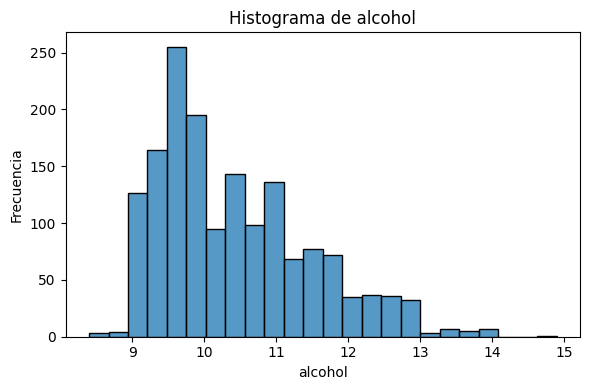
\includegraphics[width=0.9\linewidth]{images/hist_alcohol.png}
    \caption{Histograma de frecuencia vs cantidad de alcohol.}
    \label{fig:hist_alcohol}
\end{figure}

\begin{figure}[ht]
    \centering
    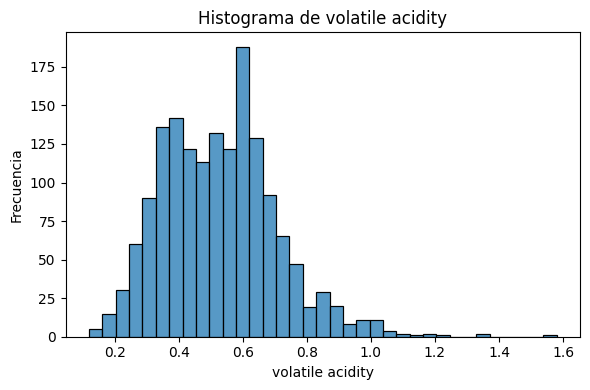
\includegraphics[width=0.9\linewidth]{images/hist_volatile_acidity.png}
    \caption{Histograma de frecuencia vs acidez volátil.}
    \label{fig:hist_volatile}
\end{figure}

Analizando la Fig.~\ref{fig:alcohol_vs_quality} podemos ver que a medida que aumenta el grado de alcohol los puntos tienden hacia la derecha indicando un aumento la calidad del vino; por otro lado en la Fig.~\ref{fig:volatile_acidity_vs_quality} se puede interpretar que a medida que la acidez volátil disminuye la calidad del vino aumenta, esto se puede apreciar al ver que la distribución de puntos tiende a la izquierda.

\begin{figure}[ht]
    \centering
    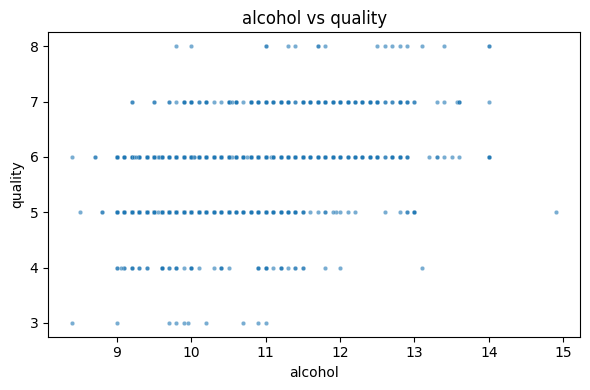
\includegraphics[width=0.9\linewidth]{images/alcohol_vs_quality.png}
    \caption{Diagrama de dispersión de alcohol vs calidad.}
    \label{fig:alcohol_vs_quality}
\end{figure}

\begin{figure}[ht]
    \centering
    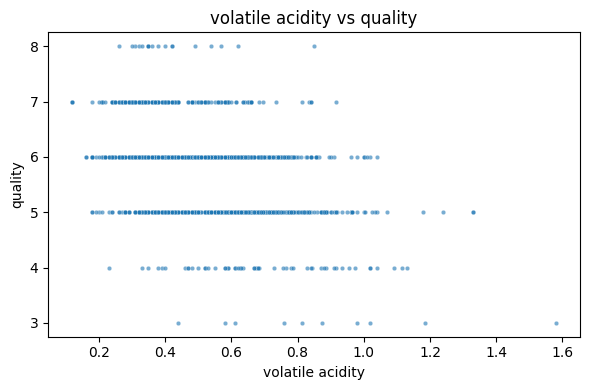
\includegraphics[width=0.9\linewidth]{images/volatile_adicity_vs_quality.png}
    \caption{Diagrama de dispersión de acidez volátil vs calidad.}
    \label{fig:volatile_acidity_vs_quality}
\end{figure}

\section{Presentación de métricas por experimento}

Se diseñó una rejilla de 10 configuraciones de hiperparámetros para la
regresión logística, variando la tasa de aprendizaje, el tamaño de lote y el
número de épocas de entrenamiento. Para cada configuración se
entrena un modelo independiente y se registran:

\begin{itemize}
    \item la pérdida de entrenamiento y de validación en cada época;
    \item las métricas finales en validación: accuracy, precisión, recall,
                F1-Score y AUC.
\end{itemize}

Las curvas \textit{Training vs Validation Loss} de los 10 experimentos se
generan en la celda 11. Una de ellas, correspondiente al experimento que obtuvo
el mejor F1-Score en validación (con \texttt{lr = 0.001}, \texttt{batch = 64}
y 50 épocas), puede verse en la Fig.~\ref{fig:loss_exp_best}.

\begin{figure}[ht]
    \centering
    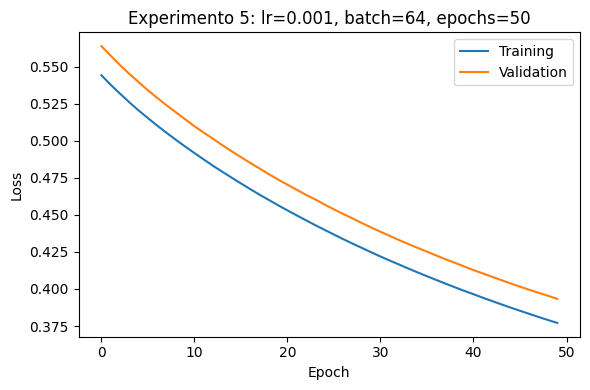
\includegraphics[width=0.9\linewidth]{images/exp5_training_validation.png}
    \caption{Curvas de pérdida de entrenamiento y validación para el experimento
    con \texttt{lr = 0.001}, \texttt{batch = 64} y 50 épocas.}
    \label{fig:loss_exp_best}
\end{figure}

En todas las configuraciones la pérdida de entrenamiento y la de validación
disminuyen de forma monótona y se mantienen cercanas entre sí, lo que sugiere
que el modelo no presenta un sobreajuste severo: no se observa que la pérdida
de validación aumente mientras la de entrenamiento sigue decreciendo. En los
experimentos con más épocas y tasa de aprendizaje moderada la separación entre
ambas curvas es algo mayor, pero sigue siendo razonable véase en la Fig.~\ref{fig:loss_exp_10}.

\begin{figure}[ht]
    \centering
    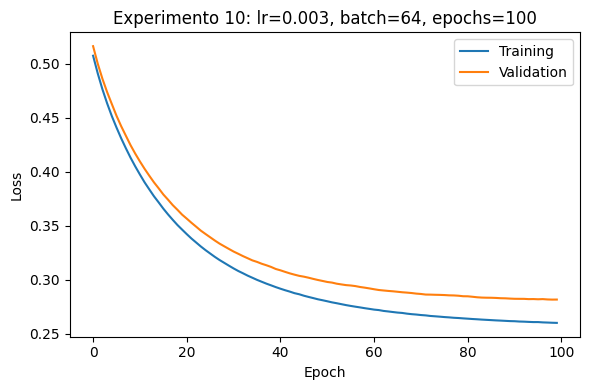
\includegraphics[width=0.9\linewidth]{images/exp10_training_validation.png}
    \caption{Curvas de pérdida de entrenamiento y validación para el experimento
    con \texttt{lr = 0.003}, \texttt{batch = 64} y 100 épocas.}
    \label{fig:loss_exp_10}
\end{figure}

Las métricas de validación de los 10 experimentos se resumen en una tabla
generada también en la celda 11 (dataframe \texttt{results\_df}). Con el
tratamiento de outliers y la partición 70/15/15, la accuracy en validación se
sitúa aproximadamente entre 0.80 y 0.89, mientras que el F1-Score oscila entre
0.30 y 0.59. El AUC se mantiene en torno a valores entre 0.78 y 0.88, lo que
indica una capacidad de discriminación razonable para distinguir vinos de
buena calidad.

El experimento con mejor F1-Score en validación corresponde ahora a la
configuración \texttt{lr = 0.001}, \texttt{batch = 64} y 50 épocas. Este
modelo se selecciona como candidato final para ser evaluado en el conjunto de
prueba.

\section{Análisis, comparación de resultados y modelo final}

Una vez identificado el mejor experimento en validación, se evalúa el modelo
resultante sobre el conjunto de prueba, manteniendo los mismos seis
predictores y el mismo umbral de decisión $0.5$ sobre la probabilidad
predicha. Con la nueva partición 70/15/15 y tras eliminar outliers, las
métricas obtenidas en test para el modelo final son, de forma aproximada, las
siguientes:
\begin{itemize}
    \item Accuracy $\approx 0.85$;
    \item Precisión $\approx 0.45$ sobre la clase ``BUENA'';
    \item Recall $\approx 0.52$;
    \item F1-Score $\approx 0.48$;
    \item AUC $\approx 0.80$.
\end{itemize}

Comparando estas métricas con las obtenidas en el conjunto de validación para
el mismo experimento (accuracy $\approx 0.89$, F1-Score $\approx 0.60$, AUC
$\approx 0.88$), se observa una ligera caída de rendimiento al pasar a prueba,
especialmente en F1 y AUC. No obstante, las diferencias no son extremas y el
comportamiento sigue siendo coherente con las curvas de pérdida, donde no se
aprecia un crecimiento sostenido de la pérdida de validación respecto a la de
entrenamiento.

Para analizar con mayor detalle los errores del modelo, se genera en la celda
11 la matriz de confusión sobre el conjunto de prueba. La Fig.~\ref{fig:cm}
muestra dicha matriz, donde la clase 1 corresponde a vinos de buena calidad y
la clase 0 a vinos normales.

\begin{figure}[ht]
    \centering
    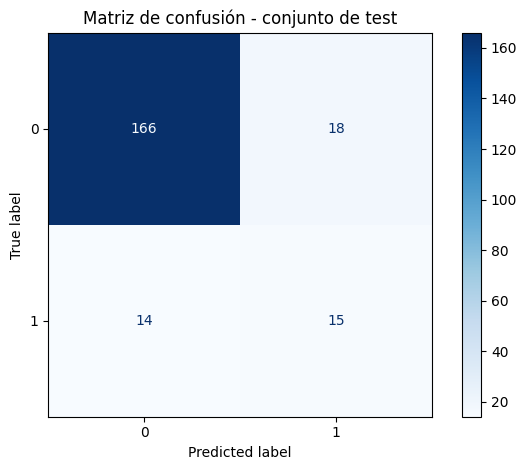
\includegraphics[width=0.9\linewidth]{images/matriz_de_confusion.png}
    \caption{Matriz de confusión del modelo final evaluado en el conjunto de
    prueba.}
    \label{fig:cm}
\end{figure}

La matriz de confusión evidencia que el modelo acierta la mayoría de los vinos
de clase 0 (baja tasa de falsos positivos) y recupera aproximadamente la mitad
de los vinos de buena calidad (recall cercano al 0.5). Dado que la clase
positiva es minoritaria, este compromiso entre precisión y recall resulta
razonable para un modelo lineal sencillo como la regresión logística.
Dependiendo de la aplicación, podría ajustarse el umbral de decisión para
privilegiar un mayor recall (aceptando más falsos positivos) o una mayor
precisión (aceptando perder algunos vinos de buena calidad).

En resumen, el modelo de regresión logística entrenado con las seis
características seleccionadas y tras el filtrado de outliers logra un
desempeño razonable en validación y prueba, sin signos claros de sobreajuste y
con una capacidad moderada para identificar vinos de buena calidad a partir de
mediciones fisicoquímicas.

\subsection{Tablas de resultados experimentales}

La Tabla~\ref{tab:val-metrics} resume las métricas de validación obtenidas en
los 10 experimentos realizados con distintas combinaciones de tasa de
aprendizaje, tamaño de lote y número de épocas. Estos valores provienen del
dataframe \texttt{results\_df} generado en la celda 11 del notebook.

\begin{table}[ht]
    \centering
    \caption{Métricas de validación por experimento de entrenamiento.}
    \label{tab:val-metrics}
    \begin{tabular}{ccccccc}
        \hline
        Exp. & $lr$ & batch & epochs & Acc & Prec & F1 \\
        \hline
        1 & 0.0000 & 32  &  50 & 0.830 & 0.426 & 0.526 \\
        2 & 0.0000 & 32  &  50 & 0.811 & 0.351 & 0.394 \\
        3 & 0.0010 & 32  &  50 & 0.863 & 0.500 & 0.408 \\
        4 & 0.0030 & 32  &  50 & 0.868 & 0.545 & 0.300 \\
        5 & 0.0010 & 64  &  50 & 0.887 & 0.586 & 0.586 \\
        6 & 0.0030 & 64  &  50 & 0.858 & 0.474 & 0.375 \\
        7 & 0.0010 & 128 &  50 & 0.797 & 0.370 & 0.482 \\
        8 & 0.0030 & 128 &  50 & 0.873 & 0.562 & 0.400 \\
        9 & 0.0010 & 64  & 100 & 0.882 & 0.567 & 0.576 \\
        10& 0.0030 & 64  & 100 & 0.868 & 0.545 & 0.300 \\
        \hline
    \end{tabular}
\end{table}

Además, en la Tabla~\ref{tab:best-val-test} se compara el rendimiento del
mejor experimento según el F1-Score en validación (configuración con
\texttt{lr = 0.001}, \texttt{batch = 64} y 50 épocas) frente a las métricas
obtenidas al evaluar ese mismo modelo sobre el conjunto de prueba. Los valores
de validación corresponden al diccionario \texttt{best\_by\_f1}, mientras que
los de prueba proceden de las variables \texttt{test\_accuracy},
\texttt{test\_precision}, \texttt{test\_recall}, \texttt{test\_f1} y
\texttt{test\_auc} calculadas en la celda 11.

\begin{table}[ht]
    \centering
    \caption{Comparación de métricas entre validación y prueba para el modelo
    seleccionado.}
    \label{tab:best-val-test}
    \begin{tabular}{lcc}
        \hline
        Métrica & Validación & Prueba \\
        \hline
        Accuracy   & 0.887 & 0.850 \\
        Precisión  & 0.586 & 0.455 \\
        Recall     & 0.586 & 0.517 \\
        F1-Score   & 0.586 & 0.484 \\
        AUC        & 0.878 & 0.804 \\
        \hline
    \end{tabular}
\end{table}

Se observa que las métricas en el conjunto de prueba son ligeramente inferiores
a las de validación, especialmente en términos de F1-Score y AUC. Aun así, la
caída de rendimiento es moderada y coherente con las curvas de pérdida, por lo
que no se aprecia un sobreajuste extremo y el modelo mantiene una capacidad de
generalización razonable sobre datos no vistos.

\section{Referencias}

\begin{thebibliography}{00}

\bibitem{b1} Bishop, C. M. (2006). \textit{Pattern recognition and machine learning}. Springer.

\bibitem{b2} Hastie, T., Tibshirani, R., \& Friedman, J. (2009). \textit{The elements of statistical learning: data mining, inference, and prediction} (2nd ed.). Springer.

\end{thebibliography}

\end{document}